\documentclass[10.5pt]{article}
% Shared style for the Airspace Monitor reports
\usepackage[a4paper,margin=1.9cm,top=2.25cm,bottom=2.05cm,headheight=18pt]{geometry}
\usepackage{fontspec}
\usepackage{xcolor}
\usepackage{graphicx}
\usepackage{tikz}
\usetikzlibrary{positioning,calc,shapes.geometric,backgrounds,arrows.meta}
\usepackage[most]{tcolorbox}
\usepackage{booktabs}
\usepackage{amssymb}
\usepackage{tabularx}
\usepackage{longtable}
\usepackage{array}
\usepackage{colortbl}
\usepackage{ragged2e}
\usepackage{enumitem}
\usepackage{fancyhdr}
\usepackage{fontawesome5}
\usepackage{hyperref}
\usepackage{microtype}
\usepackage{lastpage}

\definecolor{ink}{HTML}{0B1020}
\definecolor{panel}{HTML}{111A2E}
\definecolor{border}{HTML}{22304F}
\definecolor{textlight}{HTML}{E7ECF6}
\definecolor{muted}{HTML}{9AA8C2}
\definecolor{accent}{HTML}{4CC3FF}
\definecolor{violet}{HTML}{B392FF}
\definecolor{okgreen}{HTML}{2FAE78}
\definecolor{okgreenlight}{HTML}{E6F7F0}
\definecolor{warn}{HTML}{C77A00}
\definecolor{warnlight}{HTML}{FFF6E5}
\definecolor{alert}{HTML}{C94646}
\definecolor{alertlight}{HTML}{FDEEEE}
\definecolor{paper}{HTML}{F7F9FD}
\definecolor{papertext}{HTML}{1B2438}
\definecolor{papermuted}{HTML}{5B6B85}
\definecolor{lightborder}{HTML}{DCE4F2}
\definecolor{softblue}{HTML}{EAF6FF}
\definecolor{softviolet}{HTML}{F1ECFF}
\definecolor{softgrey}{HTML}{F0F3F9}

\setmainfont{Lato}
\setsansfont{Lato}
\setmonofont{Consolas}[Scale=0.92]
\renewcommand{\familydefault}{\sfdefault}
\setlength{\parindent}{0pt}
\setlength{\parskip}{5pt}
\RaggedRight
\renewcommand{\arraystretch}{1.32}
\setlength{\tabcolsep}{5pt}
\setlength{\emergencystretch}{1em}
\hypersetup{hidelinks}

\newcommand{\sechead}[1]{%
  \vspace{7pt}%
  {\color{papertext}\fontsize{17}{20}\selectfont\bfseries #1}\par
  \vspace{-2pt}{\color{accent}\rule{\linewidth}{1.3pt}}\par
  \vspace{5pt}%
}
\newcommand{\subhead}[1]{%
  \vspace{5pt}{\color{papertext}\fontsize{11.5}{14}\selectfont\bfseries #1}\par
  \vspace{1pt}%
}
\newcommand{\code}[1]{\texttt{\detokenize{#1}}}
\newcommand{\docsrc}[1]{{\scriptsize\color{papermuted}\texttt{\detokenize{#1}}}}

\newcommand{\pill}[2]{%
  \begin{tikzpicture}[baseline=(x.base)]%
    \node[fill=#1,text=white,rounded corners=2.4pt,inner sep=2.6pt,font=\scriptsize\bfseries] (x) {#2};%
  \end{tikzpicture}%
}
\newcommand{\dotok}{\textcolor{okgreen}{\faCircle}}
\newcommand{\dotwarn}{\textcolor{warn}{\faCircle}}
\newcommand{\dotbad}{\textcolor{alert}{\faCircle}}

\newtcolorbox{card}[1][]{enhanced,breakable,colback=white,colframe=lightborder,boxrule=0.6pt,arc=2.2mm,left=4mm,right=4mm,top=3mm,bottom=3mm,#1}
\newtcolorbox{accentcard}[1][]{enhanced,breakable,colback=softblue,colframe=accent,boxrule=0.8pt,arc=2.2mm,left=4mm,right=4mm,top=3mm,bottom=3mm,#1}
\newtcolorbox{warncard}[1][]{enhanced,breakable,colback=warnlight,colframe=warn,boxrule=0.8pt,arc=2.2mm,left=4mm,right=4mm,top=3mm,bottom=3mm,#1}
\newtcolorbox{badcard}[1][]{enhanced,breakable,colback=alertlight,colframe=alert,boxrule=0.8pt,arc=2.2mm,left=4mm,right=4mm,top=3mm,bottom=3mm,#1}
\newtcolorbox{violetcard}[1][]{enhanced,breakable,colback=softviolet,colframe=violet,boxrule=0.8pt,arc=2.2mm,left=4mm,right=4mm,top=3mm,bottom=3mm,#1}
\newtcolorbox{softcard}[1][]{enhanced,breakable,colback=softgrey,colframe=lightborder,boxrule=0.6pt,arc=2.2mm,left=4mm,right=4mm,top=3mm,bottom=3mm,#1}

\pagestyle{fancy}
\fancyhf{}
\fancyhead[L]{\scriptsize\color{papermuted}Airspace Monitor · Documentation Review}
\fancyhead[R]{\scriptsize\color{papermuted}30 October 2026}
\fancyfoot[L]{\scriptsize\color{papermuted}Level 1 · pre-implementation}
\fancyfoot[R]{\scriptsize\color{papermuted}\thepage\ / \pageref{LastPage}}
\renewcommand{\headrulewidth}{0.4pt}
\renewcommand{\footrulewidth}{0.4pt}
\renewcommand{\headrule}{\hbox to\headwidth{\color{lightborder}\leaders\hrule height \headrulewidth\hfill}}
\renewcommand{\footrule}{\hbox to\headwidth{\color{lightborder}\leaders\hrule height \footrulewidth\hfill}}


\pagestyle{fancy}
\fancyhf{}
\fancyhead[L]{\scriptsize\color{papermuted}Airspace Monitor · How it works}
\fancyhead[R]{\scriptsize\color{papermuted}2 November 2026}
\fancyfoot[L]{\scriptsize\color{papermuted}Level 1 · architecture and execution plan}
\fancyfoot[R]{\scriptsize\color{papermuted}\thepage\ / \pageref{LastPage}}
\renewcommand{\headrulewidth}{0.4pt}
\renewcommand{\footrulewidth}{0.4pt}

\tikzset{
  box/.style={draw=lightborder,fill=white,rounded corners=1.6pt,align=center,
    font=\scriptsize,inner sep=3.5pt,minimum height=0.85cm},
  run/.style={box,fill=softblue,draw=accent},
  plan/.style={box,fill=white,draw=papermuted,dashed},
  ext/.style={box,fill=softgrey,draw=papermuted},
  edge/.style={box,fill=softviolet,draw=violet},
  group/.style={draw=lightborder,fill=softgrey!55,rounded corners=2.4pt},
  arrow/.style={-{Latex[length=1.7mm]},draw=papermuted,line width=0.65pt},
  livearrow/.style={arrow,draw=accent,line width=0.95pt},
  dashedarrow/.style={arrow,dashed},
  label/.style={font=\tiny,text=papermuted,inner sep=1pt},
  grouplabel/.style={font=\scriptsize\bfseries,text=papermuted,anchor=west}
}

\begin{document}
\hypersetup{pdftitle={Airspace Monitor - How It Works},pdfauthor={Alek Hanusic and Daniel Csorba},pdfsubject={Architecture, data flows and the two build tracks}}

% ============================================================
% COVER
% ============================================================
\pagecolor{ink}
\color{textlight}
\thispagestyle{empty}

\begin{tikzpicture}[remember picture,overlay]
  \foreach \x in {0,...,14} {
    \draw[white,opacity=0.035,line width=0.4pt]
      ($(current page.south west)+(\x*1.55cm,0)$) -- ++(0,29.7cm);
  }
  \foreach \y in {0,...,19} {
    \draw[white,opacity=0.035,line width=0.4pt]
      ($(current page.south west)+(0,\y*1.55cm)$) -- ++(21cm,0);
  }
  \draw[accent,opacity=0.30,line width=0.8pt]
    ($(current page.north east)+(-4.8cm,-3.4cm)$) arc[start angle=205,end angle=515,radius=2.1cm];
  \node[circle,draw=accent,fill=accent!12,minimum size=1.05cm,line width=0.8pt]
    at ($(current page.north east)+(-4.8cm,-3.4cm)$) {\color{accent}\large\faPlane};
\end{tikzpicture}

\vspace*{2.0cm}
{\color{accent}\fontsize{9}{11}\selectfont\bfseries SYSTEM GUIDE \quad·\quad LEVEL 1 \quad·\quad 2 NOVEMBER 2026}

\vspace{0.5cm}
{\fontsize{38}{42}\selectfont\bfseries How Airspace Monitor Works}

\vspace{0.18cm}
{\color{textlight}\fontsize{20}{25}\selectfont Architecture, data flows and the two build tracks}

\vspace{0.8cm}
{\color{muted}\fontsize{11.2}{15.5}\selectfont
A guided tour from the collector on a home PC to the map, the arrival board and the guarded AI chat — plus a practical split of the work between Track A and Track B.\par}

\vspace{0.35cm}
{\color{muted}\fontsize{11.2}{15.5}\selectfont
This is the companion to the system documents \code{00}--\code{11}; the documents remain the source of truth.\par}

\vfill
{\color{muted}\fontsize{9}{12}\selectfont
Solid boxes = running or committed. Dashed boxes = to build before the core is complete.\\
{\color{accent}\rule{1.2cm}{1pt}}\quad The system is deliberately small: one collector, one VM, one database, one scheduler.
}

\newpage
\pagecolor{paper}
\color{papertext}

% ============================================================
% PAGE 2 — MAIN PATH
% ============================================================
\sechead{The main path}

{\small
Follow one snapshot from the sky to the browser. The top row is the collector and ingest path; the bottom row is what the platform does with the data.
}

\vspace{2pt}
\begin{center}
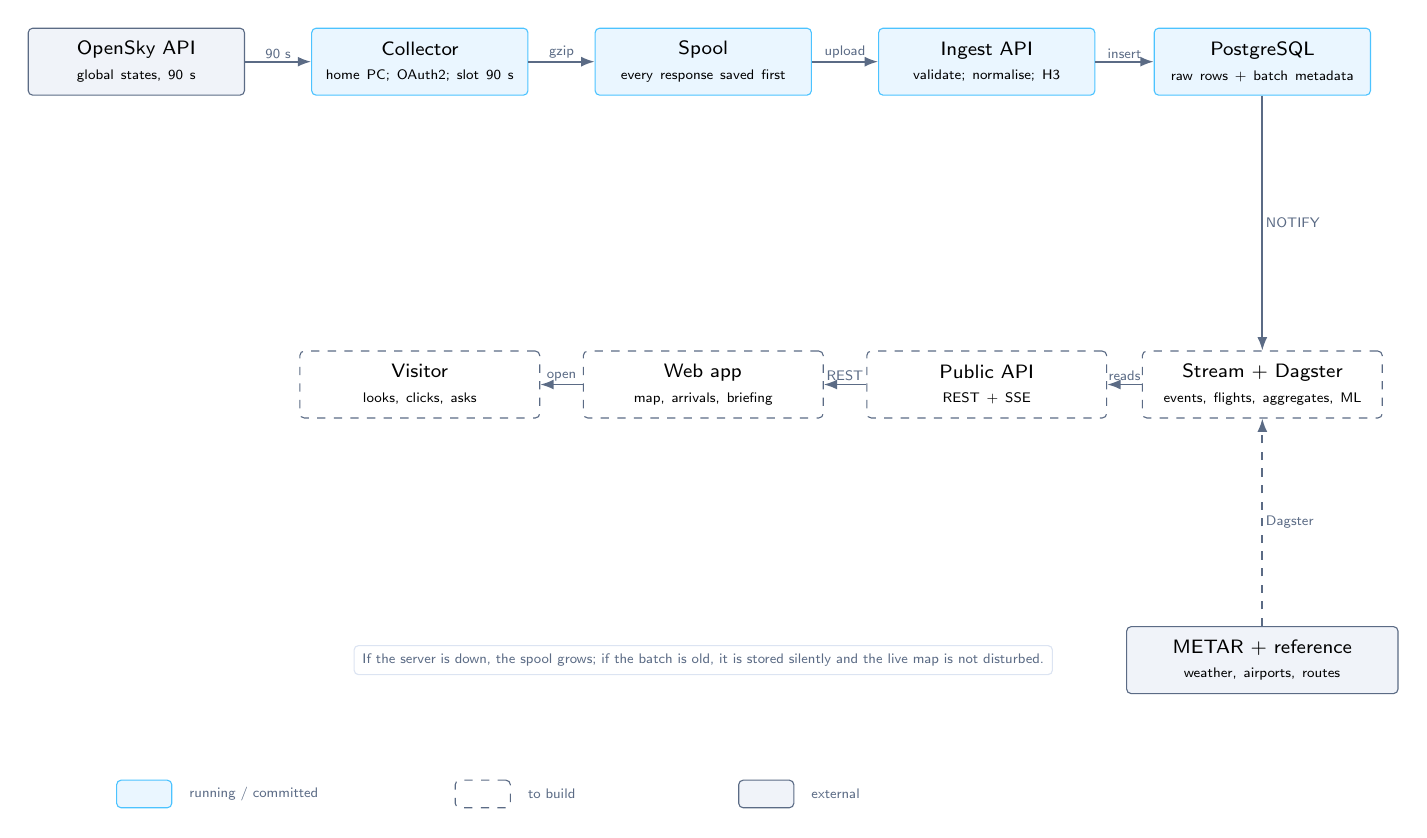
\begin{tikzpicture}[x=1cm,y=1cm]

% top row
\node[ext,text width=2.5cm] (opensky) at (1.7,14.2) {OpenSky API\\[1pt]{\tiny global states, 90 s}};
\node[run,text width=2.5cm] (collector) at (5.3,14.2) {Collector\\[1pt]{\tiny home PC; OAuth2; slot 90 s}};
\node[run,text width=2.5cm] (spool) at (8.9,14.2) {Spool\\[1pt]{\tiny every response saved first}};
\node[run,text width=2.5cm] (ingest) at (12.5,14.2) {Ingest API\\[1pt]{\tiny validate; normalise; H3}};
\node[run,text width=2.5cm] (db) at (16.0,14.2) {PostgreSQL\\[1pt]{\tiny raw rows + batch metadata}};

% bottom row (right-to-left)
\node[plan,text width=2.8cm] (process) at (16.0,10.1) {Stream + Dagster\\[1pt]{\tiny events, flights, aggregates, ML}};
\node[plan,text width=2.8cm] (api) at (12.5,10.1) {Public API\\[1pt]{\tiny REST + SSE}};
\node[plan,text width=2.8cm] (web) at (8.9,10.1) {Web app\\[1pt]{\tiny map, arrivals, briefing}};
\node[plan,text width=2.8cm] (user) at (5.3,10.1) {Visitor\\[1pt]{\tiny looks, clicks, asks}};

% arrows
\draw[arrow] (opensky) -- node[label,above]{90 s} (collector);
\draw[arrow] (collector) -- node[label,above]{gzip} (spool);
\draw[arrow] (spool) -- node[label,above]{upload} (ingest);
\draw[arrow] (ingest) -- node[label,above]{insert} (db);
\draw[arrow] (db.south) -- node[label,right]{NOTIFY} (process.north);
\draw[arrow] (process.west) -- node[label,above]{reads} (api.east);
\draw[arrow] (api.west) -- node[label,above]{REST} (web.east);
\draw[arrow] (web.west) -- node[label,above]{open} (user.east);

% side notes
\node[ext,text width=3.2cm] (metar) at (16.0,6.6) {METAR + reference\\[1pt]{\tiny weather, airports, routes}};
\draw[dashedarrow] (metar.north) -- node[label,right]{Dagster} (process.south);

\node[draw=lightborder,fill=white,rounded corners=1.5pt,align=center,font=\tiny,text=papermuted,inner sep=3pt] at (8.9,6.6) {If the server is down, the spool grows; if the batch is old, it is stored silently and the live map is not disturbed.};

% legend
\node[run,minimum width=0.7cm,minimum height=0.35cm] at (1.8,4.9) {};
\node[anchor=west,font=\tiny,text=papermuted] at (2.25,4.9) {running / committed};
\node[plan,minimum width=0.7cm,minimum height=0.35cm] at (6.1,4.9) {};
\node[anchor=west,font=\tiny,text=papermuted] at (6.55,4.9) {to build};
\node[ext,minimum width=0.7cm,minimum height=0.35cm] at (9.7,4.9) {};
\node[anchor=west,font=\tiny,text=papermuted] at (10.15,4.9) {external};
\end{tikzpicture}
\end{center}

\vspace{2pt}
\begin{softcard}
{\bfseries The one-sentence version.} A home PC turns OpenSky snapshots into durable batches; the VM turns those batches into a time-series database, flights, events, aggregates and predictions; the web app turns the latest state into a map, a board and an AI answer.
\end{softcard}

\begin{minipage}[t]{0.49\linewidth}
\begin{card}
{\bfseries What is running today (2 Nov 2026)}
\begin{itemize}[leftmargin=1.05em,itemsep=1.5pt,topsep=2pt]
  \item pc-daniel collector, spool and uploader
  \item Oracle A1 VM, Tailscale, Docker
  \item TimescaleDB + PostGIS, migrations
  \item ingest-api and collector admin CLI
  \item 8.75M state vectors and 119k flight-list rows ingested
\end{itemize}
\end{card}
\end{minipage}\hfill
\begin{minipage}[t]{0.49\linewidth}
\begin{card}
{\bfseries What the finished core adds}
\begin{itemize}[leftmargin=1.05em,itemsep=1.5pt,topsep=2pt]
  \item Aggregates, Dagster jobs, DQ, Grafana
  \item public-api, SSE, web map and panels
  \item stream-worker events and ETA inference
  \item MLflow, ETA model, route lookup
  \item briefing, guarded chat, golden-set eval
\end{itemize}
\end{card}
\end{minipage}

% ============================================================
% PAGE 3 — DEPLOYMENT VIEW
% ============================================================
\newpage
\sechead{Where everything runs}

{\small
The system spans four places: a home connection, one Oracle VM, Cloudflare's edge before a public launch, and a few external services. The table is the quick reference; the two boxes below show the current private path and the path added for public launch.
}

\vspace{2pt}
\begin{center}
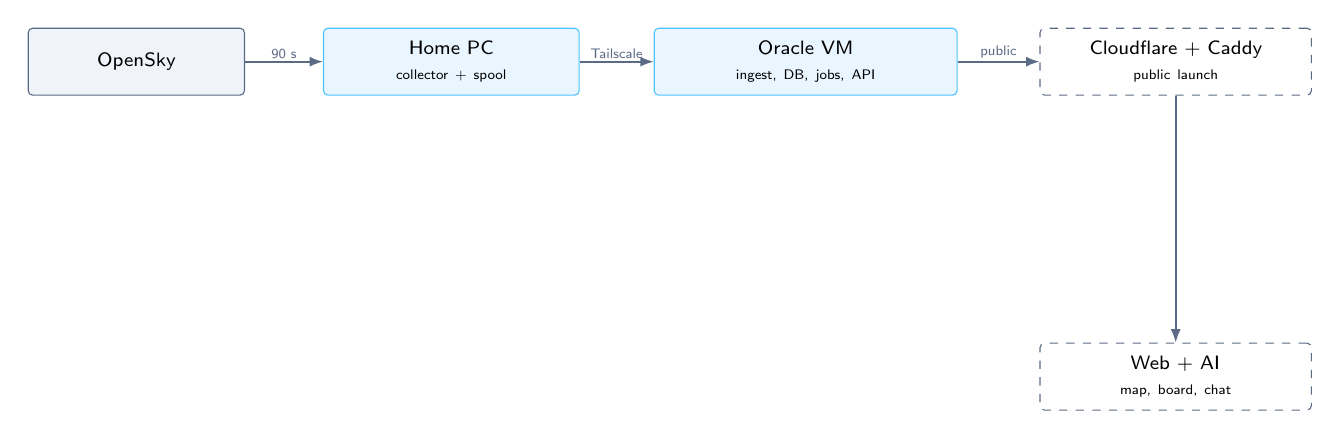
\begin{tikzpicture}[x=1cm,y=1cm]
\node[ext,text width=2.5cm] (opensky) at (1.7,15.2) {OpenSky};
\node[run,text width=3.0cm] (home) at (5.7,15.2) {Home PC\\[1pt]{\tiny collector + spool}};
\node[run,text width=3.6cm] (vm) at (10.2,15.2) {Oracle VM\\[1pt]{\tiny ingest, DB, jobs, API}};
\node[plan,text width=3.2cm] (edge) at (14.9,15.2) {Cloudflare + Caddy\\[1pt]{\tiny public launch}};
\node[plan,text width=3.2cm] (web) at (14.9,11.2) {Web + AI\\[1pt]{\tiny map, board, chat}};
\draw[arrow] (opensky) -- node[label,above]{90 s} (home);
\draw[arrow] (home) -- node[label,above]{Tailscale} (vm);
\draw[arrow] (vm) -- node[label,above]{public} (edge);
\draw[arrow] (edge.south) -- (web.north);
\end{tikzpicture}
\end{center}

\begin{tabularx}{\linewidth}{@{}p{3.0cm} p{2.8cm} X p{2.1cm}@{}}
\toprule
\textbf{Component} & \textbf{Runs on} & \textbf{Responsibility} & \textbf{Status} \\
\midrule
Collector & Home PC & Poll OpenSky on 90 s grid; spool every response; upload oldest-first; daily flight lists & Running \\
Spool + archive & Home PC / R2 & Local durability, Parquet compaction, off-PC archive & Partial \\
ingest-api & Oracle VM & Authenticate, validate, normalise, H3, insert batches idempotently & Running \\
PostgreSQL & Oracle VM & TimescaleDB + PostGIS; raw, curated, aggregates, predictions, LLM data & Running \\
stream-worker & Oracle VM & Per-snapshot squawk/go-around events and ETA inference & To build \\
Dagster & Oracle VM & Windowed jobs: flights, labels, METAR, aggregates, anomaly, briefing, DQ, backup & To build \\
public-api & Oracle VM & Read API, SSE stream, chat endpoint & To build \\
MLflow & Oracle VM & Experiment tracking and model registry; private & To build \\
Grafana & Oracle VM & Ops, data-quality and model dashboards; externally shared & To build \\
Caddy + Cloudflare & Edge & TLS, DNS, proxy, rate limits; public hostnames & Later (private now) \\
\bottomrule
\end{tabularx}

\vspace{4pt}
\begin{minipage}[t]{0.49\linewidth}
\begin{accentcard}
{\bfseries Current path (private)}
\begin{enumerate}[leftmargin=1.25em,itemsep=1.5pt,topsep=2pt]
  \item OpenSky → collector on pc-daniel
  \item collector writes gzipped batches to spool
  \item uploader posts over Tailscale to ingest-api
  \item ingest writes raw rows and batch metadata
  \item no inbound ports; SSH and admin over Tailscale
\end{enumerate}
\end{accentcard}
\end{minipage}\hfill
\begin{minipage}[t]{0.49\linewidth}
\begin{violetcard}
{\bfseries Added before public launch}
\begin{enumerate}[leftmargin=1.25em,itemsep=1.5pt,topsep=2pt]
  \item Cloudflare DNS, proxy and rate limits
  \item Caddy with Cloudflare Origin CA certificate
  \item public-api, web app and Grafana hostnames
  \item public web fetches the latest snapshot by \code{?t=}
  \item OpenSky written licence confirmed first
\end{enumerate}
\end{violetcard}
\end{minipage}

\vspace{4pt}
\begin{warncard}
{\bfseries The boundary that matters.} OpenSky sees a residential IP, not Oracle. The VM never calls OpenSky. The collector is the only component that needs the OpenSky client secret and the only one that writes the spool. The server can be down without losing already-fetched data; it catches up later.
\end{warncard}

% ============================================================
% PAGE 4 — LIVE AND BATCH FLOWS
% ============================================================
\newpage
\sechead{Two flows: live and batch}

{\small
The system has one fast path for the map and one slower path for history, models and briefings. Keeping them separate is what makes the 90-second feed cheap.
}

\vspace{2pt}
\begin{minipage}[t]{0.48\linewidth}
\begin{card}
{\bfseries Live path · every 90 s}
\vspace{3pt}
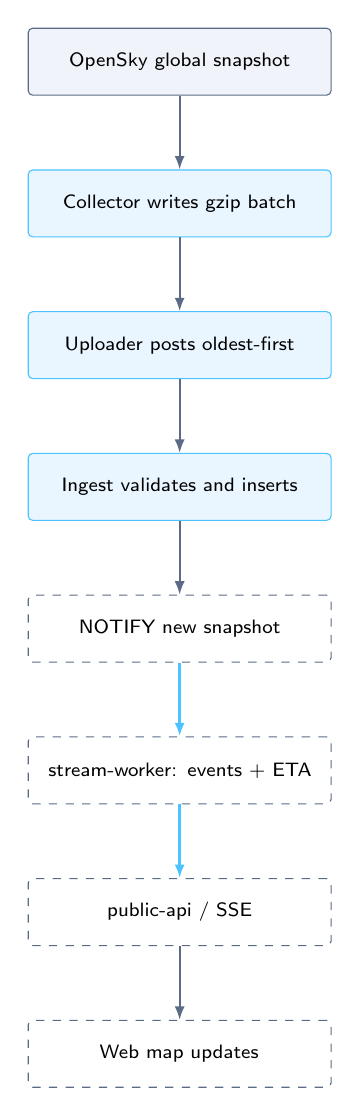
\begin{tikzpicture}[x=1cm,y=1cm,every node/.style={font=\scriptsize}]
\node[ext,text width=3.6cm] (a) at (0,0) {OpenSky global snapshot};
\node[run,text width=3.6cm] (b) at (0,-1.8) {Collector writes gzip batch};
\node[run,text width=3.6cm] (c) at (0,-3.6) {Uploader posts oldest-first};
\node[run,text width=3.6cm] (d) at (0,-5.4) {Ingest validates and inserts};
\node[plan,text width=3.6cm] (e) at (0,-7.2) {NOTIFY new snapshot};
\node[plan,text width=3.6cm] (f) at (0,-9.0) {stream-worker: events + ETA};
\node[plan,text width=3.6cm] (g) at (0,-10.8) {public-api / SSE};
\node[plan,text width=3.6cm] (h) at (0,-12.6) {Web map updates};
\draw[arrow] (a) -- (b);
\draw[arrow] (b) -- (c);
\draw[arrow] (c) -- (d);
\draw[arrow] (d) -- (e);
\draw[livearrow] (e) -- (f);
\draw[livearrow] (f) -- (g);
\draw[arrow] (g) -- (h);
\end{tikzpicture}
\end{card}
\end{minipage}\hfill
\begin{minipage}[t]{0.48\linewidth}
\begin{card}
{\bfseries Batch path · 5 min to daily}
\vspace{3pt}
\begin{tikzpicture}[x=1cm,y=1cm,every node/.style={font=\scriptsize}]
\node[plan,text width=3.6cm] (a) at (0,0) {Dagster tick};
\node[plan,text width=3.6cm] (b) at (0,-1.8) {Sessionizer: build flights};
\node[plan,text width=3.6cm] (c) at (0,-3.6) {Labels + route lookup};
\node[plan,text width=3.6cm] (d) at (0,-5.4) {CAGG refresh + baseline};
\node[plan,text width=3.6cm] (e) at (0,-7.2) {Anomaly scoring / events};
\node[plan,text width=3.6cm] (f) at (0,-9.0) {Facts → LLM briefing};
\node[plan,text width=3.6cm] (g) at (0,-10.8) {DQ + backup};
\node[plan,text width=3.6cm] (h) at (0,-12.6) {API serves history / models};
\draw[arrow] (a) -- (b);
\draw[arrow] (b) -- (c);
\draw[arrow] (c) -- (d);
\draw[arrow] (d) -- (e);
\draw[arrow] (e) -- (f);
\draw[arrow] (f) -- (g);
\draw[arrow] (g) -- (h);
\end{tikzpicture}
\end{card}
\end{minipage}

\vspace{4pt}
\begin{softcard}
{\bfseries Catch-up path.} If the server or network is down, the collector keeps writing to \code{spool/pending}. The uploader retries with back-off and drains oldest-first when the server returns. Batches older than the 10-minute live window are stored but do not notify, so the map and stream are never rewound; \code{agg_backfill_refresh} materialises the affected days later. Manual \code{flights_rebuild} and \code{events_rebuild} cover the derived tables.
\end{softcard}

\vspace{3pt}
\begin{softcard}
{\bfseries Why the split matters.} The live path has a hard latency budget: a new snapshot should reach the map in seconds, and only the latest snapshot matters. The batch path can take minutes and can look backwards. Sharing one database but not one latency budget is what keeps the 90-second feed cheap and the history correct.
\end{softcard}

\newpage
\sechead{Failure and recovery}

{\small
The system is designed to keep the last good state visible and to recover data later, rather than trying to pretend nothing happened.
}

\vspace{2pt}
\begin{center}
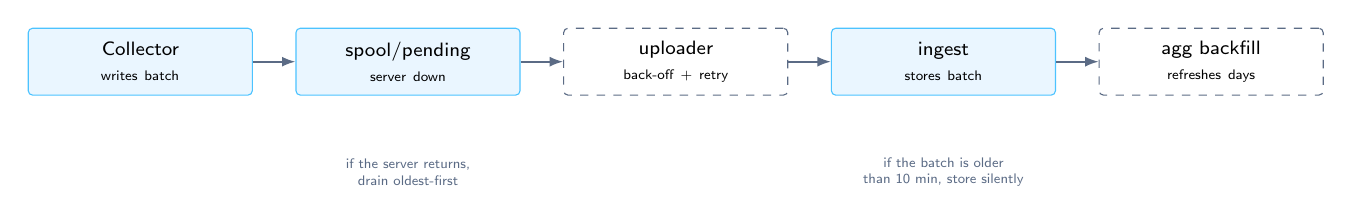
\begin{tikzpicture}[x=1cm,y=1cm]
\node[run,text width=2.6cm] (collector) at (1.6,8.2) {Collector\\[1pt]{\tiny writes batch}};
\node[run,text width=2.6cm] (pending) at (5.0,8.2) {spool/pending\\[1pt]{\tiny server down}};
\node[plan,text width=2.6cm] (retry) at (8.4,8.2) {uploader\\[1pt]{\tiny back-off + retry}};
\node[run,text width=2.6cm] (ingest) at (11.8,8.2) {ingest\\[1pt]{\tiny stores batch}};
\node[plan,text width=2.6cm] (refresh) at (15.2,8.2) {agg backfill\\[1pt]{\tiny refreshes days}};
\draw[arrow] (collector) -- (pending);
\draw[arrow] (pending) -- (retry);
\draw[arrow] (retry) -- (ingest);
\draw[arrow] (ingest) -- (refresh);
\node[font=\tiny,text=papermuted,align=center] at (5.0,6.8) {if the server returns,\\drain oldest-first};
\node[font=\tiny,text=papermuted,align=center] at (11.8,6.8) {if the batch is older\\than 10 min, store silently};
\end{tikzpicture}
\end{center}

\begin{tabularx}{\linewidth}{@{}p{3.9cm} p{6.4cm} X@{}}
\toprule
\textbf{Trigger} & \textbf{Immediate behaviour} & \textbf{Recovery} \\
\midrule
OpenSky 429 or timeout & Skip the slot, spool a failed envelope, obey \code{Retry-After}; the next slot is unaffected & Next slot; failed envelope explains the gap \\
Server unreachable & Pending spool grows; uploader backs off; map stays on the last good snapshot & Drain spool oldest-first; no live rewind \\
Batch older than 10 min & Stored silently; no SSE and no stream-worker & \code{agg_backfill_refresh}; manual re-score if needed \\
Stream worker down & Notifications are not durable; recent events can be missed & Manual \code{events_rebuild} over the window \\
Data-quality failure & \code{dq_fail} event and Grafana red status & Investigate; the UI does not hide the gap \\
Home PC off & No new snapshots; the last snapshot ages out of the live window & Resume when the PC returns; gap is visible \\
\bottomrule
\end{tabularx}

\vspace{4pt}
\begin{minipage}[t]{0.49\linewidth}
\begin{card}
{\bfseries What to monitor}
\begin{itemize}[leftmargin=1.05em,itemsep=1.5pt,topsep=2pt]
  \item \code{/health}: DB reachable; last snapshot age
  \item \code{/stats}: aircraft now, collectors online, rows today
  \item Grafana: slot coverage, gaps, ingest lag, credits
  \item DQ table: pass / warn / fail per check
  \item Spool: pending count, oldest pending age
\end{itemize}
\end{card}
\end{minipage}\hfill
\begin{minipage}[t]{0.49\linewidth}
\begin{warncard}
{\bfseries What is intentionally not automatic}
\begin{itemize}[leftmargin=1.05em,itemsep=1.5pt,topsep=2pt]
  \item Anomaly history is not re-scored when late data arrives.
  \item Stream events missed during a long outage need \code{events_rebuild}.
  \item Flights touched by late points need \code{flights_rebuild}.
  \item These are documented limits, not silent failures.
\end{itemize}
\end{warncard}
\end{minipage}

% ============================================================
% PAGE 6 — DATA PLATFORM
% ============================================================
\newpage
\sechead{Inside the data platform}

{\small
The database is organised as a medallion pipeline: raw data first, then curated entities, then aggregates and predictions. The chat is allowed to see only the final read-only views.
}

\vspace{2pt}
\begin{center}
\begin{tikzpicture}[x=1cm,y=1cm]
\node[run,text width=3.1cm] (raw) at (8.5,15.0) {raw · bronze\\[1pt]{\tiny state vectors; OpenSky flight lists}};
\node[plan,text width=3.1cm] (core) at (8.5,11.4) {core · silver\\[1pt]{\tiny flights; METAR; events}};
\node[plan,text width=3.1cm] (agg) at (4.1,7.8) {agg · gold\\[1pt]{\tiny 15-min density; coverage; baseline}};
\node[plan,text width=3.1cm] (ml) at (8.5,7.8) {ml · gold\\[1pt]{\tiny anomalies; ETA; destinations}};
\node[plan,text width=3.1cm] (llm) at (12.9,7.8) {llm · gold\\[1pt]{\tiny briefings; chat; v\_ views}};
\node[ext,text width=3.1cm] (ref) at (3.2,12.8) {ref\\[1pt]{\tiny airports; runways; aircraft; routes}};
\node[ext,text width=3.1cm] (ops) at (13.8,12.8) {ops\\[1pt]{\tiny batches; jobs; DQ; model runs}};

\draw[arrow] (raw) -- (core);
\draw[arrow] (core.south west) -- (agg.north east);
\draw[arrow] (core) -- (ml);
\draw[arrow] (agg) -- (ml);
\draw[arrow] (core.south east) -- (llm.north west);
\draw[arrow] (ml) -- (llm);
\draw[dashedarrow] (ref.south east) -- (core.west);
\draw[dashedarrow] (ops.south west) -- (raw.east);

\node[font=\tiny,text=papermuted,align=center] at (8.5,5.9) {raw → core → agg / ml → llm\\the chat reads only \code{llm.v_*}};
\end{tikzpicture}
\end{center}

\begin{tabularx}{\linewidth}{@{}p{2.2cm} p{5.7cm} p{4.0cm} X@{}}
\toprule
\textbf{Schema} & \textbf{Main tables} & \textbf{Written by} & \textbf{Used for} \\
\midrule
\code{raw} & \code{state_vectors}, \code{opensky_flights} & ingest-api & source of truth; archives \\
\code{ref} & airports, runways, aircraft, airlines, countries, callsign routes & Dagster & joins; route lookup; wind \\
\code{core} & flights, METAR, events & stream-worker, Dagster & the product's entities \\
\code{agg} & \code{traffic_h3_15m}, coverage, baseline & Timescale, Dagster & density and anomalies \\
\code{ml} & anomalies, ETA, destination predictions & stream-worker, Dagster & map, board, card \\
\code{llm} & briefings, chat log, \code{v_*} views & API, Dagster & briefing and chat \\
\code{ops} & collectors, batches, jobs, DQ, model runs & all services & operations and audit \\
\bottomrule
\end{tabularx}

\vspace{4pt}
\begin{softcard}
{\bfseries Keys are the contract.} \code{batch_id} makes uploads idempotent. \code{dedupe_key} keeps events unique. \code{flight_id} is assigned once and never changes. Natural keys and explicit job windows let every scheduled job be re-run safely.
\end{softcard}

% ============================================================
% PAGE 7 — SCHEDULE
% ============================================================
\newpage
\sechead{What runs when}

{\small
The live path is continuous; the rest is a set of windows. The cadence is chosen around OpenSky credits, the 90 s source, and how quickly the product needs to react.
}

\vspace{2pt}
\begin{center}
\begin{tikzpicture}[x=1cm,y=1cm]
\draw[arrow] (0,4.2) -- (17,4.2);
\foreach \h/\lab in {0/00,6/06,12/12,18/18,24/24} {
  \draw[papermuted,line width=0.5pt] (\h*17/24,4.0) -- (\h*17/24,4.4);
  \node[font=\tiny,text=papermuted,anchor=north] at (\h*17/24,3.8) {\lab:00};
}
\foreach \t in {0.35,0.7,1.4,2.8,4.2,5.6,5.95} {
  \fill[accent] (\t*17/24,4.2) circle (1.7pt);
}
\draw[accent,line width=0.8pt] (0.35*17/24,4.75) -- (5.95*17/24,4.75);
\node[font=\tiny,text=accent,anchor=south] at (3.15*17/24,4.85) {daily batch window};
\node[font=\tiny,text=papermuted] at (9.0,3.15) {dots = daily jobs; exact times in the table};
\end{tikzpicture}
\end{center}

\begin{tabularx}{\linewidth}{@{}p{2.1cm} p{5.2cm} X@{}}
\toprule
\textbf{Cadence} & \textbf{Job / action} & \textbf{Why this cadence} \\
\midrule
90 s & Collector fetch + ingest + stream-worker + SSE & OpenSky credit budget: 960 global calls/day at 4 credits \\
5 min & \code{flights_sessionizer}, destination inference, gap check & flights and the card need to feel current \\
15 min (+2) & \code{anomaly_scoring} on the closed bucket & heatmap and anomaly events \\
30 min & \code{metar_fetch}, \code{llm_briefing} & weather and briefing are slower-moving \\
Hourly & \code{agg_backfill_refresh}, \code{dq_checks} & late data and health \\
Daily & baseline (02:00), backup (04:00), flight lists (06:00), labels (08:00), routes (08:30), compaction (00:30), R2 (01:00) & one pass over the previous day \\
Weekly & \code{train_eta} Sunday 03:00 & enough new arrivals to retrain \\
\bottomrule
\end{tabularx}

\vspace{4pt}
\begin{minipage}[t]{0.49\linewidth}
\begin{accentcard}
{\bfseries The live promise}
\begin{itemize}[leftmargin=1.05em,itemsep=1.5pt,topsep=2pt]
  \item At most one snapshot every 90 s.
  \item The map is never rewound to old data.
  \item The last good snapshot stays visible during an outage.
  \item Every gap is measurable.
\end{itemize}
\end{accentcard}
\end{minipage}\hfill
\begin{minipage}[t]{0.49\linewidth}
\begin{warncard}
{\bfseries The batch promise}
\begin{itemize}[leftmargin=1.05em,itemsep=1.5pt,topsep=2pt]
  \item Every job has an explicit \code{[start, end)} window.
  \item Every job is idempotent for that window.
  \item Late data is caught up, not hidden.
  \item Training never runs in CI; only on the server.
\end{itemize}
\end{warncard}
\end{minipage}

% ============================================================
% PAGE 8 — ML FLOWS
% ============================================================
\newpage
\sechead{How the ML works}

{\small
Three different jobs: unusual traffic (unsupervised), arrival time (supervised quantile regression), and destination (a deterministic route lookup in the core, with a re-ranker as stretch).
}

\vspace{2pt}
\begin{center}
\begin{tikzpicture}[x=1cm,y=1cm,every node/.style={font=\scriptsize}]
% headers
\node[font=\scriptsize\bfseries,text=accent] at (2.8,1.0) {Unusual traffic};
\node[font=\scriptsize\bfseries,text=accent] at (8.5,1.0) {Arrival time (ETA)};
\node[font=\scriptsize\bfseries,text=accent] at (14.2,1.0) {Destination};

% anomaly column
\node[run,text width=4.0cm] (a1) at (2.8,-0.4) {raw state vectors};
\node[plan,text width=4.0cm] (a2) at (2.8,-2.0) {15-min H3 density};
\node[plan,text width=4.0cm] (a3) at (2.8,-3.6) {hour-of-week baseline};
\node[plan,text width=4.0cm] (a4) at (2.8,-5.2) {robust z-score + persistence};
\node[plan,text width=4.0cm] (a5) at (2.8,-6.8) {anomalies + events};
\node[plan,text width=4.0cm] (a6) at (2.8,-8.4) {heatmap / briefing facts};
\draw[arrow] (a1) -- (a2); \draw[arrow] (a2) -- (a3);
\draw[arrow] (a3) -- (a4); \draw[arrow] (a4) -- (a5); \draw[arrow] (a5) -- (a6);

% ETA column
\node[run,text width=4.0cm] (e1) at (8.5,-0.4) {raw states + METAR};
\node[plan,text width=4.0cm] (e2) at (8.5,-2.0) {flights + labels};
\node[plan,text width=4.0cm] (e3) at (8.5,-3.6) {feature extraction};
\node[plan,text width=4.0cm] (e4) at (8.5,-5.2) {weekly LightGBM training};
\node[plan,text width=4.0cm] (e5) at (8.5,-6.8) {MLflow champion};
\node[plan,text width=4.0cm] (e6) at (8.5,-8.4) {stream inference → p10/p50/p90};
\node[plan,text width=4.0cm] (e7) at (8.5,-10.0) {arrivals board};
\draw[arrow] (e1) -- (e2); \draw[arrow] (e2) -- (e3);
\draw[arrow] (e3) -- (e4); \draw[arrow] (e4) -- (e5);
\draw[arrow] (e5) -- (e6); \draw[arrow] (e6) -- (e7);

% destination column
\node[run,text width=4.0cm] (d1) at (14.2,-0.4) {flight lists + Zenodo};
\node[plan,text width=4.0cm] (d2) at (14.2,-2.0) {callsign → route lookup};
\node[plan,text width=4.0cm] (d3) at (14.2,-3.6) {destination inference};
\node[plan,text width=4.0cm] (d4) at (14.2,-5.2) {top-3 in aircraft card};
\node[plan,text width=4.0cm] (d5) at (14.2,-6.8) {re-ranker (stretch)};
\draw[arrow] (d1) -- (d2); \draw[arrow] (d2) -- (d3);
\draw[arrow] (d3) -- (d4); \draw[dashedarrow] (d4) -- (d5);
\end{tikzpicture}
\end{center}

\begin{tabularx}{\linewidth}{@{}p{3.0cm} p{4.0cm} p{4.0cm} X@{}}
\toprule
\textbf{Model} & \textbf{Baseline} & \textbf{Evaluation} & \textbf{Success} \\
\midrule
Unusual traffic v1 & median/MAD by hour of week & synthetic injection; flags/day; real-event list & useful precision/recall, not a fixed score \\
ETA & B0 distance/speed; B1 distance-band median & time-based hold-out; MAE; p10–p90 coverage & p50 MAE beats B1 \\
Destination lookup & nearest airport ahead & top-1 / top-3 at 10/50/90\% progress & beat nearest-airport baseline \\
\bottomrule
\end{tabularx}

\begin{softcard}
{\bfseries Train and serve use the same feature code.} Feature functions live in \code{libs/airspace_common} and \code{ml/}; training extracts Parquet with DuckDB, serving reads Postgres. MLflow stores the run, the metrics and the artifact. Only the \code{champion} alias is served; MLflow stays private.
\end{softcard}

% ============================================================
% PAGE 9 — LLM FLOWS
% ============================================================
\newpage
\sechead{How the LLM layer works}

{\small
Two features, one rule: the model writes prose, but it does not invent facts and it does not get unrestricted SQL.
}

\vspace{2pt}
\begin{minipage}[t]{0.48\linewidth}
\begin{card}
{\bfseries Briefing · every 30 min}
\vspace{3pt}
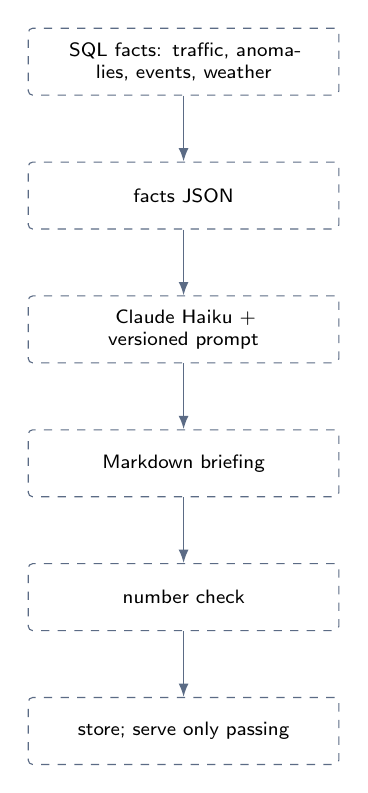
\begin{tikzpicture}[x=1cm,y=1cm,every node/.style={font=\scriptsize}]
\node[plan,text width=3.7cm] (a) at (0,0) {SQL facts: traffic, anomalies, events, weather};
\node[plan,text width=3.7cm] (b) at (0,-1.7) {facts JSON};
\node[plan,text width=3.7cm] (c) at (0,-3.4) {Claude Haiku + versioned prompt};
\node[plan,text width=3.7cm] (d) at (0,-5.1) {Markdown briefing};
\node[plan,text width=3.7cm] (e) at (0,-6.8) {number check};
\node[plan,text width=3.7cm] (f) at (0,-8.5) {store; serve only passing};
\draw[arrow] (a) -- (b); \draw[arrow] (b) -- (c);
\draw[arrow] (c) -- (d); \draw[arrow] (d) -- (e);
\draw[arrow] (e) -- (f);
\end{tikzpicture}
\end{card}
\end{minipage}\hfill
\begin{minipage}[t]{0.48\linewidth}
\begin{card}
\vspace{3pt}
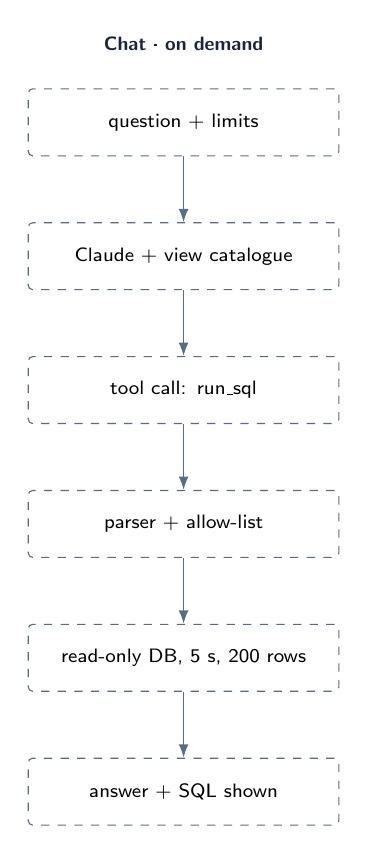
\begin{tikzpicture}[x=1cm,y=1cm,every node/.style={font=\scriptsize}]
\node[font=\scriptsize\bfseries,text=papertext] at (0,1.0) {Chat · on demand};
\node[plan,text width=3.7cm] (a) at (0,0) {question + limits};
\node[plan,text width=3.7cm] (b) at (0,-1.7) {Claude + view catalogue};
\node[plan,text width=3.7cm] (c) at (0,-3.4) {tool call: run\_sql};
\node[plan,text width=3.7cm] (d) at (0,-5.1) {parser + allow-list};
\node[plan,text width=3.7cm] (e) at (0,-6.8) {read-only DB, 5 s, 200 rows};
\node[plan,text width=3.7cm] (f) at (0,-8.5) {answer + SQL shown};
\draw[arrow] (a) -- (b); \draw[arrow] (b) -- (c);
\draw[arrow] (c) -- (d); \draw[arrow] (d) -- (e);
\draw[arrow] (e) -- (f);
\end{tikzpicture}
\end{card}
\end{minipage}

\vspace{4pt}
\begin{minipage}[t]{0.49\linewidth}
\begin{accentcard}
{\bfseries Guardrails}
\begin{itemize}[leftmargin=1.05em,itemsep=1.5pt,topsep=2pt]
  \item \code{llm_readonly}: SELECT only on \code{llm.v_*}.
  \item One SELECT, allow-listed functions, no INTO/locking.
  \item 5 s statement timeout; 200-row cap; 3 tool calls.
  \item SQL always shown; rejected queries count as a call.
  \item 10 questions/hour/IP; 200/day; \$40/month cap.
\end{itemize}
\end{accentcard}
\end{minipage}\hfill
\begin{minipage}[t]{0.49\linewidth}
\begin{warncard}
{\bfseries Why the number check exists}
The briefing may only use numbers from the facts JSON. Every number in the output is matched back to a fact (with rounding); a failed briefing is stored but never served. The previous passing briefing stays visible. This is the cheapest defence against a confident, wrong sentence.
\end{warncard}
\end{minipage}

% ============================================================
% PAGE 10 — TWO TRACKS
% ============================================================
\newpage
\sechead{The two build tracks}

{\small
The split is by ownership, not by layer. Track A makes the data trustworthy; Track B makes it useful and visible. They meet at the data model and the API contract, and both review each other's PRs.
}

\vspace{2pt}
\begin{minipage}[t]{0.48\linewidth}
\begin{accentcard}
{\bfseries Track A · Data platform}
\begin{itemize}[leftmargin=1.05em,itemsep=2pt,topsep=2pt]
  \item Collector, spool, uploader, flight lists
  \item ingest-api, auth, idempotency, H3
  \item DB, migrations, roles, retention, backups
  \item Dagster jobs, DQ, Grafana ops
  \item CI/CD, VM, Tailscale, R2, restore drill
\end{itemize}
\vspace{2pt}
{\small\textbf{Delivers:} a database and a job graph that Track B can trust.}
\end{accentcard}
\end{minipage}\hfill
\begin{minipage}[t]{0.48\linewidth}
\begin{violetcard}
{\bfseries Track B · Product and ML}
\begin{itemize}[leftmargin=1.05em,itemsep=2pt,topsep=2pt]
  \item public-api, SSE, web app, map layers
  \item ETA model, arrivals board, model cards
  \item Anomaly scoring, heatmap, events
  \item Destination lookup, aircraft card
  \item Briefing, chat, guardrails, golden-set eval
\end{itemize}
\vspace{2pt}
{\small\textbf{Delivers:} the visible product and the measurable ML/LLM results.}
\end{violetcard}
\end{minipage}

\vspace{4pt}
\begin{softcard}
{\bfseries Shared surface: contract first.} \code{docs/03-data-model.md} defines the tables; \code{docs/05-api-contract.md} defines the endpoints. Change the contract first, then the code, and update the doc in the same PR. The unusual-traffic model is explicitly shared: Track A builds the aggregate and baseline, Track B builds scoring, the heatmap and the evaluation.
\end{softcard}

\begin{tabularx}{\linewidth}{@{}p{3.2cm} p{6.2cm} X@{}}
\toprule
\textbf{Handoff} & \textbf{Track A gives} & \textbf{Track B needs it for} \\
\midrule
Data model & \code{raw}, \code{core}, \code{agg}, \code{ml}, \code{llm} tables and keys & API queries, model labels, chat views \\
Aggregates & \code{agg.traffic_h3_15m}, coverage, baseline & anomaly scoring and heatmap \\
Flights & sessionizer, labels, route lookup & ETA training, arrivals board, card \\
API contract & endpoint shapes and units & web app, SSE, chat UI \\
Ops & health, DQ, backups, deploy & a product that can be trusted and shown \\
\bottomrule
\end{tabularx}

\vspace{4pt}
\begin{minipage}[t]{0.49\linewidth}
\begin{card}
{\bfseries Current state (from 11-tasks)}
Track A is ahead: collector, VM, database, migrations, ingest-api and uploader are running; 8.75M state vectors are stored. Track B is mostly at the starting line: API, web, stream worker, Dagster, ML and LLM are still to build.
\end{card}
\end{minipage}\hfill
\begin{minipage}[t]{0.49\linewidth}
\begin{warncard}
{\bfseries Open decision O1}
Who owns Track A and Track B is still undecided. Decide it in week 0; the work split only works if each person has a clear primary track and both review the other's PRs.
\end{warncard}
\end{minipage}

% ============================================================
% PAGE 11 — MILESTONES
% ============================================================
\newpage
\sechead{Milestones and the critical path}

{\small
The two tracks run in parallel, but they do not run independently: Track B's API and map need Track A's database, flights and aggregates. The critical path is collector → ingest → database → flights/labels → ETA → arrivals board.
}

\vspace{2pt}
\begin{center}
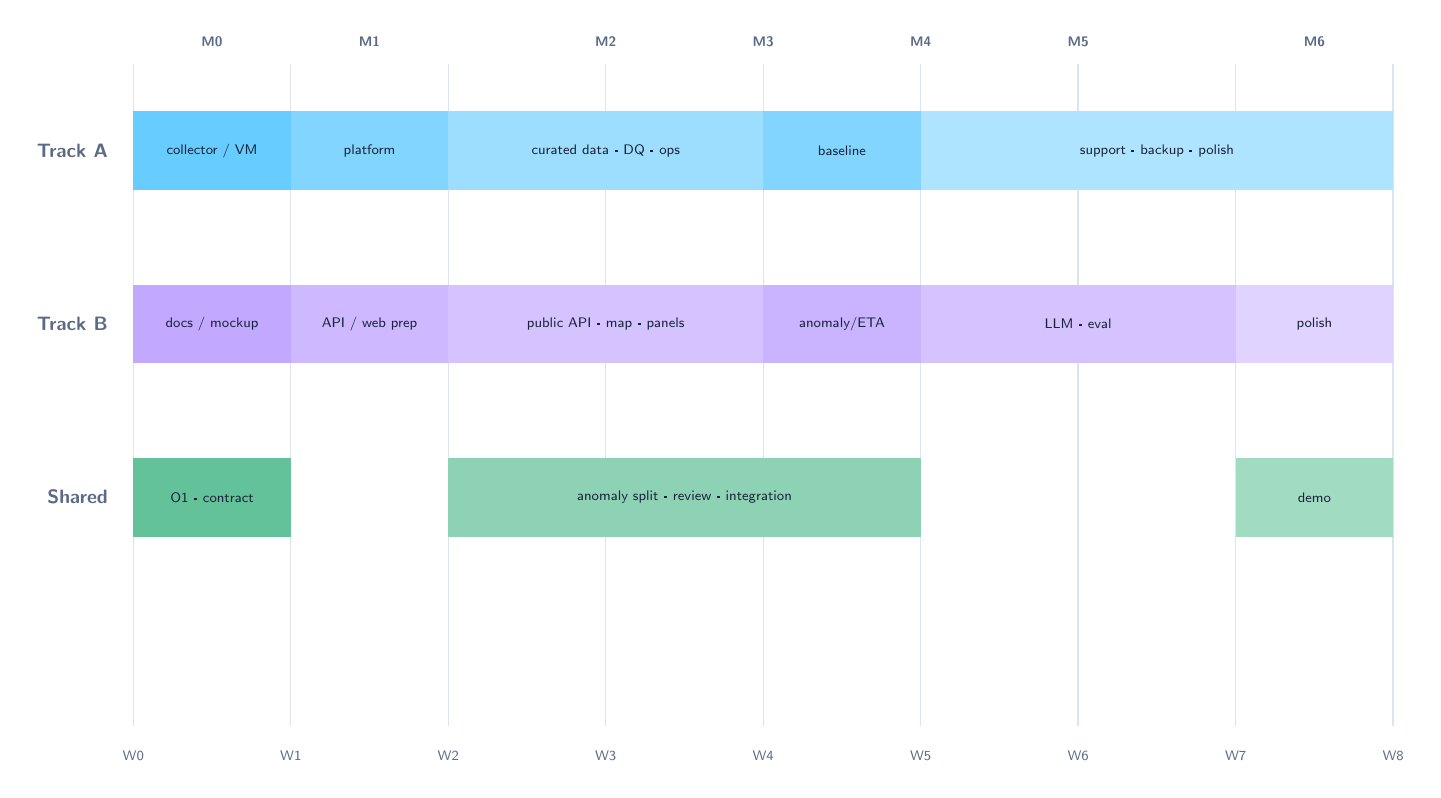
\begin{tikzpicture}[x=1cm,y=1cm]
% week axis
\foreach \w in {0,...,8} {
  \draw[lightborder,line width=0.5pt] (\w*2,0.2) -- (\w*2,8.6);
  \node[font=\tiny,text=papermuted,anchor=north] at (\w*2,0.0) {W\w};
}
% row labels
\node[font=\scriptsize\bfseries,text=papermuted,anchor=east] at (-0.2,7.5) {Track A};
\node[font=\scriptsize\bfseries,text=papermuted,anchor=east] at (-0.2,5.3) {Track B};
\node[font=\scriptsize\bfseries,text=papermuted,anchor=east] at (-0.2,3.1) {Shared};

% A bars
\fill[accent!85] (0,7.0) rectangle (2,8.0); \node[font=\tiny,text=papertext] at (1,7.5) {collector / VM};
\fill[accent!70] (2,7.0) rectangle (4,8.0); \node[font=\tiny,text=papertext] at (3,7.5) {platform};
\fill[accent!55] (4,7.0) rectangle (8,8.0); \node[font=\tiny,text=papertext] at (6,7.5) {curated data · DQ · ops};
\fill[accent!70] (8,7.0) rectangle (10,8.0); \node[font=\tiny,text=papertext] at (9,7.5) {baseline};
\fill[accent!45] (10,7.0) rectangle (16,8.0); \node[font=\tiny,text=papertext] at (13,7.5) {support · backup · polish};

% B bars
\fill[violet!80] (0,4.8) rectangle (2,5.8); \node[font=\tiny,text=papertext] at (1,5.3) {docs / mockup};
\fill[violet!65] (2,4.8) rectangle (4,5.8); \node[font=\tiny,text=papertext] at (3,5.3) {API / web prep};
\fill[violet!55] (4,4.8) rectangle (8,5.8); \node[font=\tiny,text=papertext] at (6,5.3) {public API · map · panels};
\fill[violet!70] (8,4.8) rectangle (10,5.8); \node[font=\tiny,text=papertext] at (9,5.3) {anomaly/ETA};
\fill[violet!55] (10,4.8) rectangle (14,5.8); \node[font=\tiny,text=papertext] at (12,5.3) {LLM · eval};
\fill[violet!40] (14,4.8) rectangle (16,5.8); \node[font=\tiny,text=papertext] at (15,5.3) {polish};

% shared bars
\fill[okgreen!75] (0,2.6) rectangle (2,3.6); \node[font=\tiny,text=papertext] at (1,3.1) {O1 · contract};
\fill[okgreen!55] (4,2.6) rectangle (10,3.6); \node[font=\tiny,text=papertext] at (7,3.1) {anomaly split · review · integration};
\fill[okgreen!45] (14,2.6) rectangle (16,3.6); \node[font=\tiny,text=papertext] at (15,3.1) {demo};

% milestone labels
\foreach \x/\m in {1/M0,3/M1,6/M2,8/M3,10/M4,12/M5,15/M6} {
  \node[font=\tiny\bfseries,text=papermuted,anchor=south] at (\x,8.7) {\m};
}
\end{tikzpicture}
\end{center}

\begin{tabularx}{\linewidth}{@{}p{2.4cm} p{5.3cm} X@{}}
\toprule
\textbf{Milestone} & \textbf{Track A} & \textbf{Track B} \\
\midrule
M0 · Foundations & collector v0, VM, DB & docs, mockup, contract review \\
M1 · Platform & ingest, migrations, Dagster, DQ, Grafana, CI, backup & API contract, web shell prep \\
M2 · Live map & stream worker, METAR, network & public API, map, events, deploy \\
M3 · Curated data & sessionizer, labels, routes, ref data & ETA data prep; anomaly design \\
M4 · ML & baseline, MLflow & anomaly, ETA, destination, model cards \\
M5 · LLM & support, views, deploy & briefing, chat, guardrails, eval \\
M6 · Polish & restore drill, docs & README, demo video, final report \\
\bottomrule
\end{tabularx}

\vspace{4pt}
\begin{minipage}[t]{0.49\linewidth}
\begin{accentcard}
{\bfseries Next five actions}
\begin{enumerate}[leftmargin=1.25em,itemsep=1.5pt,topsep=2pt]
  \item Decide O1: who owns A and B.
  \item Finish M0.13/M0.14: 48 h check, measured rows/day.
  \item Land M1.10--M1.13: aggregates, compression, Dagster, Grafana.
  \item Land M1.14--M1.16: CI, deploy, backup + restore drill.
  \item Start Track B's API and map against the stable contract.
\end{enumerate}
\end{accentcard}
\end{minipage}\hfill
\begin{minipage}[t]{0.49\linewidth}
\begin{warncard}
{\bfseries What not to do}
\begin{itemize}[leftmargin=1.05em,itemsep=1.5pt,topsep=2pt]
  \item Do not start stretch before M5 is green.
  \item Do not open a public URL before the OpenSky licence is confirmed.
  \item Do not add a fourth ML model.
  \item Do not let M6 become feature time.
\end{itemize}
\end{warncard}
\end{minipage}

\end{document}
